\input{pack.tex}

\title{\LARGE \textbf{MiniRT} - Notes}
\author{\large Lucie Le Briquer}
\date{\today}

\begin{document}
\maketitle
\tableofcontents
\newpage
\section{Génération des rayons}
\begin{center}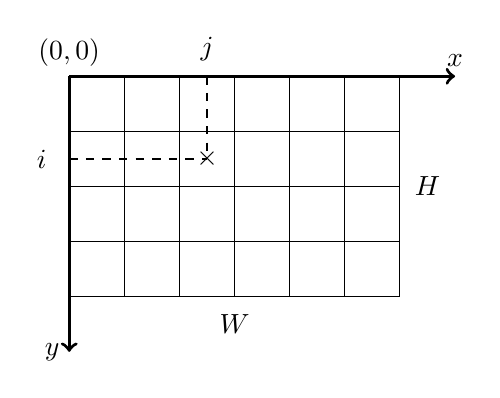
\begin{tikzpicture}[scale=0.7]
	\draw[step=1.0,black,thin] (0,0) grid (6,4);
	\draw[->,very thick] (0,4)--(7,4);
	\draw (7,4) node[above]{$x$};
	\draw[->,very thick] (0,4)--(0,-1);
	\draw (0,-1) node[left]{$y$};
	\draw (0,4) node[left,above]{$(0,0)$};
	\draw (2.5,2.5) node{$\times$};
	\draw (3,-0.5) node{$W$};
	\draw (6.5,2) node{$H$};
	\draw (-0.5,2.5) node{$i$};
	\draw (2.5,4.5) node{$j$};
	\draw[dashed] (0,2.5)--(2.5,2.5);
	\draw[dashed] (2.5,4)--(2.5,2.5);
\end{tikzpicture}
\hspace{1cm}
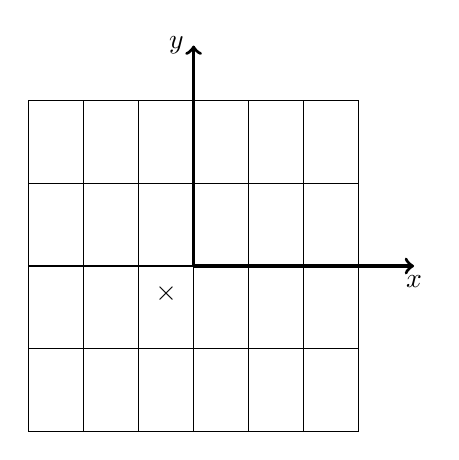
\begin{tikzpicture}[scale=0.7]
	\draw[step=1,yscale=1.5,black,thin] (0,0) grid (6,4);
	\draw[->,very thick] (3,3)--(7,3);
	\draw (7,3) node[below]{$x$};
	\draw[->,very thick] (3,3)--(3,7);
	\draw (3,7) node[left]{$y$};
	\draw (2.5,2.5) node{$\times$};
\end{tikzpicture}\end{center}
\dd\ni On cherche a remplir l'image pixel par pixel, on a $i$ correspondant a la
ligne du pixel et $j$ a sa colonne. On va d'abord normaliser les coordonnees
selon la largeur et la hauteur de l'ecran pour travailler avec une image carree.
On note :
$$\text{pixNorm}_x=\frac{j + 0.5} W \etsp\text{pixNorm}_y\frac{i + 0.5} H$$
\ni On effectue ensuite une translation pour centrer le repere sur le milieu de
l'ecran ainsi qu'une inversion de l'axe $y$. Ainsi :
$$\text{pixScreen}_x=2 \times\text{pixNorm}_x -1 \etsp \text{pixScreen}_y = 1 -
2\times \text{pixNorm}_y$$


\newpage
\section{Rotation de la caméra}
\newpage
\section{Interaction rayon-sphère}
\newpage
\section{Interaction rayon-plan}
\newpage
\section{Interaction rayon-triangle}
\newpage
\section{Interaction rayon-carré}
\newpage
\section{Interaction rayon-cylindre}
\ni Soit $(o,X,Y,Z)$ le repère du cylindre $\Cl$. Le point $p\in\Cl$ ssi
$$x_p^2 + y_p^2 = r^2\etsp|z_p|\leq\frac h 2$$
\ni avec $(x_p,y_p,z_p)$ les coordonnées de $p$ dans le repère du
cylindre. Pour déterminer les vecteurs $(X,Y,Z)$ il suffit d'utiliser la même
construction de base vue précédemment avec comme axe de départ l'axe du cylindre.
\img{0.2}{cylindre}
\dd Le point $p$ est de la forme $o_R + \bt d_R$ où $o_R$ est l'origine du rayon et
$d_R$ sa direction. Ainsi :
$$x_p = \lng p - o, X\rng = \bt\scl{d_R, X} + \scl{o_r - o, X}$$
$$y_p = \lng p - o, Y\rng = \bt\scl{d_R, Y} + \scl{o_r - o, Y}$$
Donc,
\begin{align*}
	x_p^2 + y_p^2 = &\left(\scl{d_R,X}^2 + \scl{d_r,Y}^2\right) \bt^2\\
		&+2\left(\scl{d_R,X}\scl{o_R-o,X}+\scl{d_R,Y}\scl{o_R-o,Y}\right) \bt \\
		&+\left(\scl{o_R-o, X}^2 + \scl{o_R-o,Y}^2\right)
\end{align*}
\ni$\bt$ vérifie donc une équation du second degré $a\bt^2+b\bt+c=0$ avec :
$$\sys{a = \scl{d_R,X}^2 + \scl{d_r,Y}^2\\\\
b = 2\left(\scl{d_R,X}\scl{o_R-o,X}+\scl{d_R,Y}\scl{o_R-o,Y}\right) \\\\
c = \scl{o_R-o, X}^2 + \scl{o_R-o,Y}^2 - r^2
}$$
\ni Il ne reste plus qu'à vérifier que pour un des deux $\bt$ on obtient
un point $p$ vérifiant $|z_p|\leq\frac h 2$ sachant que :
$$z_p = \lng p - o, Z\rng = \bt\scl{d_R, Z} + \scl{o_r - o, Z}$$

\end{document}
